\chapter{\new{Fundamental Mechanisms for Geo-Distributed Operation of Platform Services}
\soutnew{Necessary Mechanisms for Geo-Distributed Operation of Platform}}
\label{sec:mechanisms}

%\section{Introduction}
The challenges imposed by the peculiar characteristics of a geo-distributed Edge infrastructure and situation-awareness applications on the design of control plane policies for platform services necessitate the introduction of novel mechanisms to address them. This dissertation proposes three key mechanisms to address these challenges - Dynamic Spatial Context Management, Network Proximity Estimation and End-to-End Application Monitoring. 
\par The Dynamic Spatial Context Management mechanism allows the control plane of platform services to maintain a frequently updated view of the spatial context of system entities such as application instances, data-items and end-clients. This spatial context information is used to make control plane policy decisions, such as mapping a client to an application instance and determining the set of clients that need to share data for inter-client coordination. The objectives of these control plane policies is to ensure that the spatial affinity requirement of an application is fulfilled, as described in \cref{sec:spatial_affinity}.
\par While the Dynamic Spatial Context Management mechanism is used to establish logical connectivity between system entities based on spatial proximity, it is not responsible for mapping those system entities on to the physical infrastructure - a problem that requires taking into account the  heterogeneity in infrastructure topology and latency requirements of applications. The Network Proximity Estimation mechanism allows control plane policies to estimate the network latency between physical nodes in the infrastructure that can be used for the placement of system entities such that applications' latency requirements are satisfied. 
\par Finally, the continuous execution of applications requires the control planes of platform services to monitor the end-to-end latency experienced by each application instance, that includes queuing and computation delays as well as communication delays between different entities. The End-to-End Monitoring mechanisms allows the control plane policies to obtain an aggregated view of the various component latencies making up the end-to-end observed latency so that a violation of the application's requirements can be detected. The end-to-end view of observed latencies also enables root-cause analysis techniques to identify the source of the performance violation and trigger the appropriate reconfiguration action to alleviate it. 
\par In this chapter, we will discuss the three mechanisms proposed in this dissertation in detail. We first present the infrastructure and workload scenario that has been considered to motivate the problems solved by these mechanisms and to design the experimental settings. Then, for each mechanism, we will first describe the objective of the mechanism, enumerate examples of control plane policies that will benefit from it, present the abstractions exposed to the control plane policies, and why previous approaches at attaining this objective are not sufficient. Finally, we demonstrate the use of these abstractions for building useful control plane policies that can support the efficient operation of platform services on a realistic Edge infrastructure against a workload of situation-awareness applications. 

\section{Infrastructure Topology and Client Workload considered}
\label{sec:nep_infra_topology}
\par To make the case for the mechanisms proposed in this dissertation, we utilize the dataset \cite{xu2021cloud} characterizing the Edge cloud service of Alibaba Cloud, both at the infrastructure and workload level. At the infrastructure level, it provides detailed information about the number of Edge sites in each city of China and the network provider owning them, the number and size of physical machines in each Edge site and the network \gls{rtt} between sites. At the workload level, the dataset contains information about the number and size of \glspl{vm} hosted by each physical machine at different sites and the CPU utilization of each VM. For evaluations in this chapter, we choose the city of Shanghai as the one offering situation-awareness applications to its residents (which is just for clarity of exposition as the evaluation methodology can easily be extended to include application clients in other cities). We simulate client activity (including mobility) in the city of Shanghai ourselves, since the Edge dataset \cite{xu2021cloud} does not provide client activity information. The network connectivity between a client and an Edge site is determined by the location of the client and the geographical areas covered by each Edge site in Shanghai.
%To determine the network connectivity between a client and Edge site, it is important to know which cell towers are served by a given Edge site, or in other words, the geographical coverage of each Edge site. 
To estimate the geographical coverage of each Edge site, the precise geographical location of Edge sites and their connectivity with cell towers are needed. However, the dataset only provides a city-level granularity of Edge site locations. Hence, to estimate their precise geo-locations, we gather the locations of cell towers owned by the different network providers from CellMapper \cite{cellmapper}, perform k-means clustering on them and obtain the likely locations of the Edge sites. The number of k-means clusters for each network provider's cell tower clustering is made equal to the number of Edge sites owned by that provider in Shanghai (from the dataset). Upon obtaining the locations of Edge sites using clustering, we need to assign resource capacity to each site for which we again use the Alibaba Edge Node Service dataset, specifically the information about resource capacity of each Edge site. To map the resource capacity from the dataset to an Edge site location extracted via clustering, we assign the most resource-rich site's resource capacity in the dataset to the Edge site location that has the maximum number of cell towers in its cluster, and so on. \cref{fig:shanghai_infra} illustrates the infrastructure topology, with the locations of cell towers and Edge sites marked. In addition to Edge sites within Shanghai with precise locations, the physical infrastructure considered in our evaluations also consists of Edge sites in other cities of China. Each Edge site outside Shanghai is significantly farther away from any client considered in the workload (compared to sites within Shanghai), and therefore the city-level coarse-grained location provided by the dataset works for such a site.
\begin{figure}
\centering
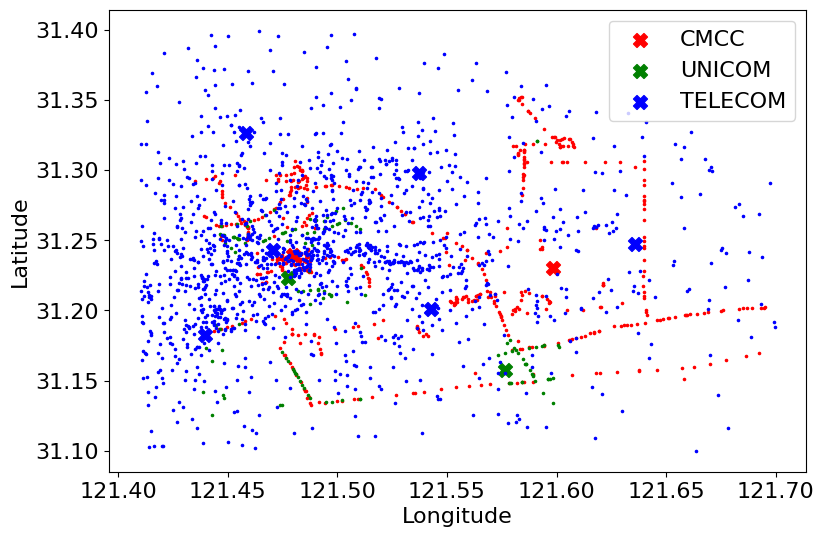
\includegraphics[width=0.5\textwidth]{figures/mechanisms/infrastructure.png}
\caption{Edge infrastructure of the city of Shanghai that is under consideration in this chapter. The crosses denote Edge site locations, while the dots denote cell tower locations. The different colors represent the three telecom providers in Shanghai, namely CMCC, China Telecom and Unicom.}
\label{fig:shanghai_infra}
\end{figure}

\section{Dynamic Spatial Management Mechanism}
\label{sec:spatial_ctx_mgmt}

Situation-awareness applications, such as collaborative autonomous driving and \gls{uav} swarm navigation, interact with the physical environment, by sensing data and performing actions on it. Typically, there are many clients of the same application operating in a common geographical space. In such a setting, a client's processing logic can benefit by incorporating information extracted from other clients' sensed data. For a given client, the set of other clients from which it needs sensor data depends on the location of clients, the size of their sensor range and the area of interest of the given client. The \gls{aoi} of a client is defined as the geographical region whose data it is interested in receiving. The sensing range of a client depends on the sensor hardware used, e.g., \gls{lidar}, camera, etc. The size of the Area-of-Interest depends on the nature of the application. For instance, since vehicles in a city are not expected to move at speeds higher than, say, 25 miles per hour (in urban cities in USA), the size of \gls{aoi} of vehicular clients for the collaborative perception application is bounded (e.g., 150 meters x 150 meters in the TalkyCars system \cite{talkycars}). There exists only a finite region around a given vehicle that would contain any interesting event for that vehicle.
\begin{figure}
\centering
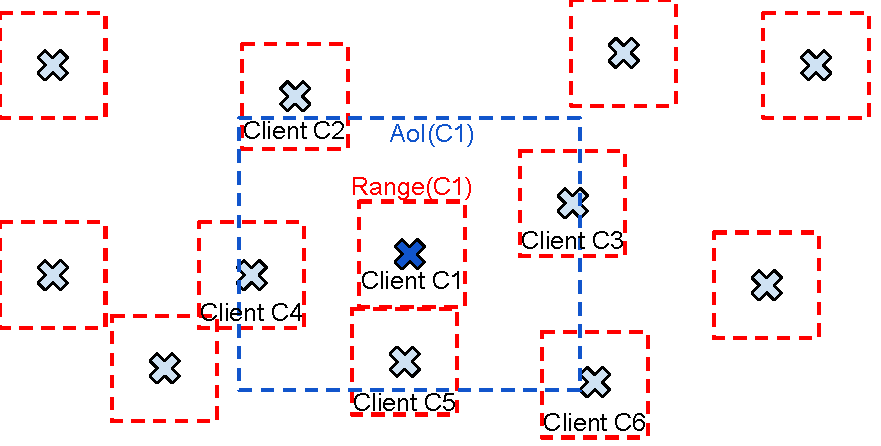
\includegraphics[width=0.75\textwidth]{figures/mechanisms/spatial_ctx_mgmt/aoi_range.pdf}
\caption{An exemplary spatial distribution of situation-awareness application clients overlaid on two-dimensional space. The sensing range of clients is shown as a red dashed rectangle around the client's location. In addition, the Area-of-Interest of client C1 is shown.}
\label{fig:aoi_range}
\end{figure}
\cref{fig:aoi_range} shows a typical arrangement of clients in geographical space with the sensing range of each client marked in red and the \gls{aoi} of one of the clients (C1) marked in blue. Each client senses data from the environment within its range and the application instance serving it generates actionable information from the sensed data. The application instance serving client C1 is interested in receiving all actionable information about the geographical region within the bounding-box of C1's \gls{aoi}. Hence, the application instance serving C1 needs to receive processed information from all other application instances that are serving those clients whose range overlaps with the AoI of C1. 

\begin{figure}
\centering
\begin{subfigure}{0.45\textwidth}
  \centering
  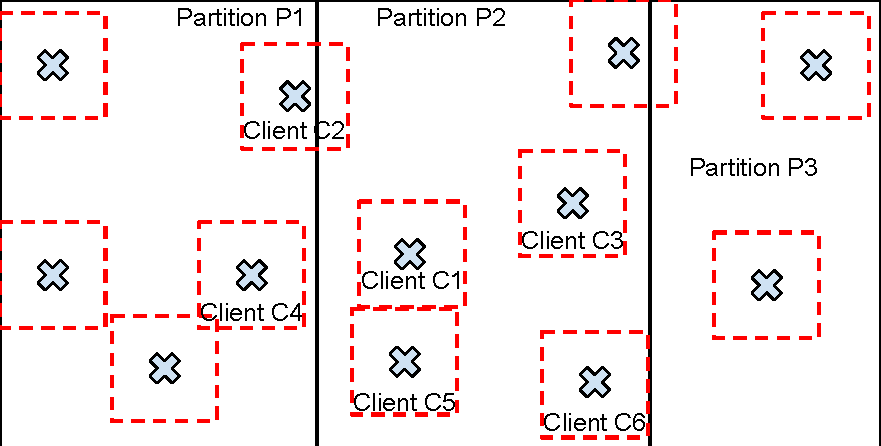
\includegraphics[width=\linewidth]{figures/mechanisms/spatial_ctx_mgmt/aoi_range_partition.pdf}
  \caption{An example partitioning of geographical space. Each partition is to be managed by a distinct application component. The important point to note is that each partition is not self-sufficient, but rather relies on information from other partitions as well. The data-dependence between partitions results from the fact that the \gls{aoi} of clients inside a given partition overlaps with the range of clients in other partitions.}
  \label{fig:aoi_range_partition}
\end{subfigure}%
~~~
\begin{subfigure}{0.45\textwidth}
  \centering
  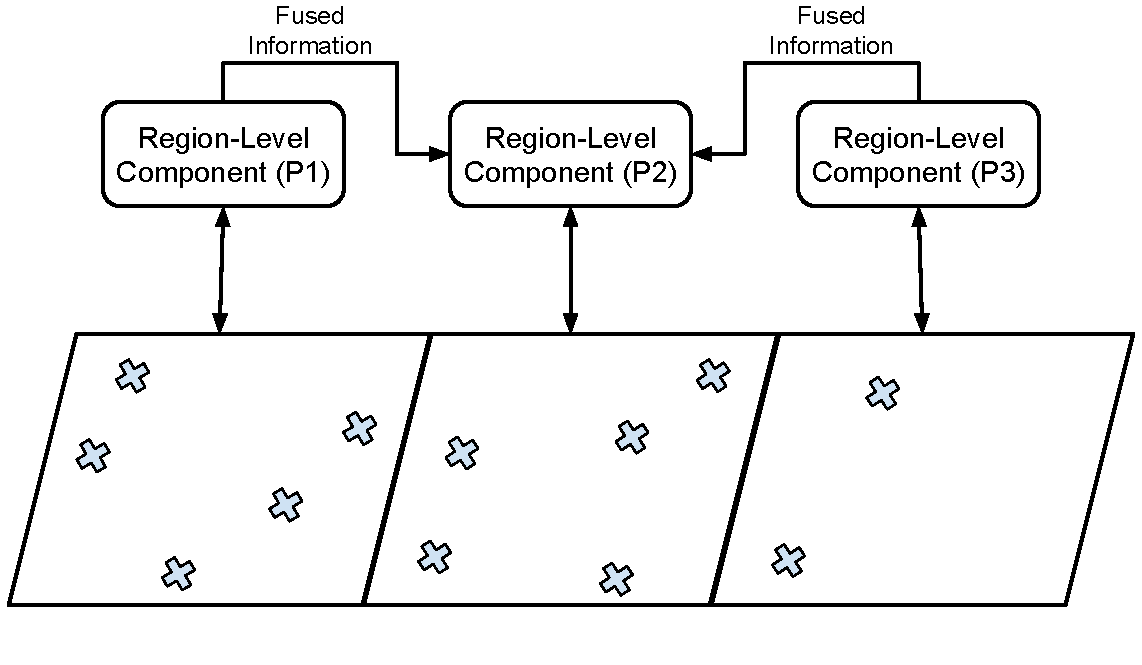
\includegraphics[width=\linewidth]{figures/mechanisms/spatial_ctx_mgmt/aoi_range_partition_mapping.pdf}
  \caption{Clients in each spatial partition are mapped to a unique region-level component that is responsible for fusing the information extracted from each individual client.}
  \label{fig:aoi_range_partition_mapping}
\end{subfigure}
\caption{Illustration of partitioning of geographical space to support large-scale deployment of situation-awareness applications that require coordination among clients.}
\label{fig:spatial_partitioning}
\end{figure}

An intuitive way of modeling these applications was discussed earlier in \cref{sec:app_model_compute}, wherein a region-level component is responsible for fusing the information extracted from multiple clients to realize inter-client coordination. However, in a large-scale geo-distributed deployment of such applications, a single region-level component would be insufficient to serve all the clients - because of scalability limitations in its implementation, resource constraints on the Edge site hosting it, or both \cite{talkycars}. Hence, to support a large number of clients, multiple instances of the region-level component are maintained as shown in \cref{fig:spatial_partitioning}, with each instance serving a distinct partition of the entire geographical area. All clients within a given spatial partition should be served by the same region-level instance, thus enabling inter-client coordination among all clients within that partition. Due to the inherent mobility of clients and the fact that the spatial partitioning is not necessarily aligned with the sensing range of each client, a client's \gls{aoi} can overlap with another client's range that is located in a different partition. For example, in \cref{fig:aoi_range_partition} client C1's \gls{aoi} overlaps with the range of client C4, however C1 and C4 belong to partitions P2 and P1 respectively. To make sure that information from client C4 is taken into account while processing the sensor data of client C1, the region-level component instance serving client C1 receives a stream of fused information from the instance serving client C4, as shown in \cref{fig:aoi_range_partition_mapping}. 

\par For situation-awareness applications that require inter-client coordination, mapping clients to region-level component instances needs to be done by taking into account the spatial context of clients (denoted by their location) and that of the region-level application component instances (denoted by spatial partition they are meant to serve). Information sharing between region-level instances is also dictated by the spatial context of the different instances and the range and \gls{aoi} of clients served by those instances, as shown in \cref{fig:spatial_data_sharing}. 

\begin{figure}
\centering
\begin{subfigure}{0.4\textwidth}
  \centering
  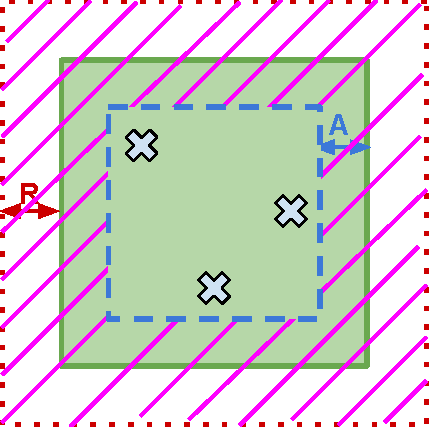
\includegraphics[width=\linewidth]{figures/mechanisms/spatial_ctx_mgmt/out_data.pdf}
  \label{fig:spatial_ctx_out_data}
  \caption{An illustration of the information generated by a given region-level component instance that needs to be shared with other instances.}
\end{subfigure}%
~~~
\begin{subfigure}{0.4\textwidth}
  \centering
  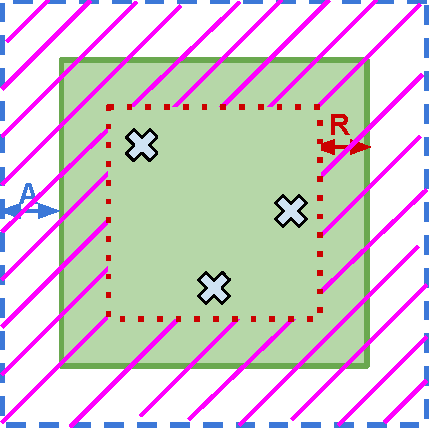
\includegraphics[width=\linewidth]{figures/mechanisms/spatial_ctx_mgmt/in_data.pdf}
  \caption{An illustration of the information needed by a region-level application component from other application instances. }
  \label{fig:spatial_ctx_in_data}
\end{subfigure}
\caption{The shaded regions in both images show the data that needs to be shared with other region-level instances (\cref{fig:spatial_ctx_out_data}) and that needs to be received from other instances (\cref{fig:spatial_ctx_in_data}). The $R$ denotes the size of sensing range, while $A$ represents the size of \gls{aoi} of each client. The shaded area represents the maximum extent of information that needs to be shared/received for any possible client location. In \cref{fig:spatial_ctx_out_data}, it is assumed that the recipient clients are located just outside the green region, while sending clients are located just inside the green region. Similarly, in \cref{fig:spatial_ctx_in_data}, it is assumed that the recipient clients within the green region are present right at the boundary, while the source clients are located just outside of the green region.}
\label{fig:spatial_data_sharing}
\end{figure}
Thus, to ensure that each client is served by an application instance specific to its spatial context and that application instances are able to share relevant data among each other, it is imperative to treat the spatial context of clients, application components and data-items as first-class attributes. 
\par The main challenge in doing so is to handle continuous client mobility, that results in the \gls{aoi} and spatial context of each client to change continuously. Hence, a static mapping of clients to application instances would result in frequent violations of the spatial affinity requirement, wherein a client would be communicating with application instances that serve a different spatial region than the one in which the client is located. Similarly, the set of data-items that a client's application instance is interested in also changes along with client mobility. Furthermore, given the continuous mobility of clients, workload skews are common - caused due to a large number of clients accumulating in a particular spatial partition, e.g., in the event of a surge in vehicular traffic in a city's downtown area due to a concert. Due to limited resource capacity of edge resources, such a workload skew can result in a performance degradation on the application instance serving that spatial partition. Therefore, spatial workload skews necessitate the monitoring and remapping of geographical regions to applications instances and data-items, so that the skews can be minimized and performance degradations can be avoided.

\subsection{Control plane actions that need this mechanism}
There are two main actions taken by the control planes of platform services that require spatial context information of clients and compute and data components:
\par \noindent \textbf{Dynamic Client-to-Application Mapping. } Situation-awareness applications require that a client be connected to a region-level application component instance that is assigned to the spatial partition within which the client is currently located. A metric that quantifies the goodness of this mapping is Spatial Alignment, that measures how many of the expected clients that should have been mapped to an application component are actually mapped. The Spatial Alignment metric for spatial partition $A$ is quantified in \cref{eq:spatial_alignment}.
\begin{equation}
SA \left( A \right) = \dfrac{\text{max. clients in }A\text{ served by the same app instance}}{\text{number of clients in }A}
\label{eq:spatial_alignment}
\end{equation}
The control plane policy for client-to-application mapping would ideally ensure the spatial alignment metric for all spatial partitions to be 1.0, meaning that all clients that are currently located in a given spatial partition $A$ are mapped to the same application instance.

\par \noindent \textbf{Area-of-Interest Queries. } Clients and application components need to query data-items whose spatial context overlaps with the querying entity's \gls{aoi}. This query is served by the control plane that evaluates the spatial context overlap with the querying entity's \gls{aoi} and returns a list of satisfying data-items. We use a metric called \gls{aoi} Satisfaction Rate to quantify the goodness of the query result, as shown in \cref{eq:aoi_sat_rate}.
\begin{equation}
\text{AoI Satisfaction Rate} = \dfrac{|\{ e: e \text{ is returned by query  and } e \in AoI \}|}{|\{ e: e \in AoI \}|}
\label{eq:aoi_sat_rate}
\end{equation}
Ideally the control plane policy for evaluating these queries should be able to achieve an \gls{aoi} Satisfaction Rate of 1.0.

\subsection{Limitations of previous work in implementing policies}
\label{sec:spatial_ctx_prev_work}
Contemporary Edge computing solutions do not allow coordination among application components that are deployed across multiple Edge sites \cite{gabriel, azure_iot_edge}. Hence, a client $c$ that is mapped to an Edge site $E$ can only coordinate with other clients that are also mapped to the site $E$. Similarly, $c$ can only discover other system entities (data-items and application instances) on the site $E$. We consider 2 high-level approaches in previous work to map clients to Edge sites - mapping each client to the geographically closest site (GeoDist) (as in L{\"a}hderanta et al. \cite{lahderanta2021edge}) and to the site with smallest \gls{rtt} from the client (RTT) (as in Saurez et al. \cite{foglets}). In the following evaluations, we show how both these approaches are deficient in satisfying the spatial alignment requirement of client-to-application mapping as well as serving Area-of-Interest based queries.

\begin{figure}
\centering
\begin{subfigure}{0.45\textwidth}
  \centering
  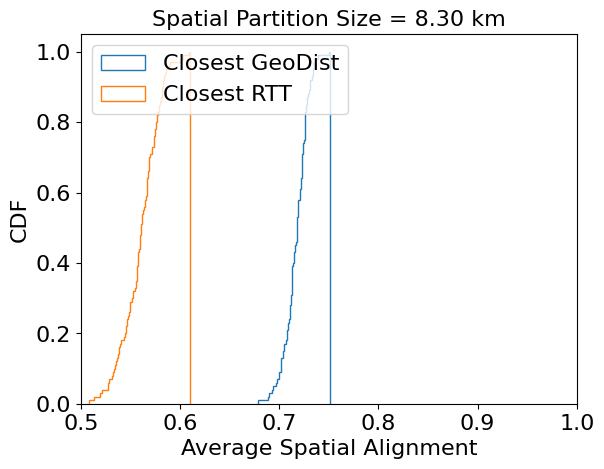
\includegraphics[width=\linewidth]{figures/mechanisms/spatial_ctx_mgmt/spatial_alignment_randomized_4_rows.png}
  \caption{}
\end{subfigure}%
\begin{subfigure}{0.45\textwidth}
  \centering
  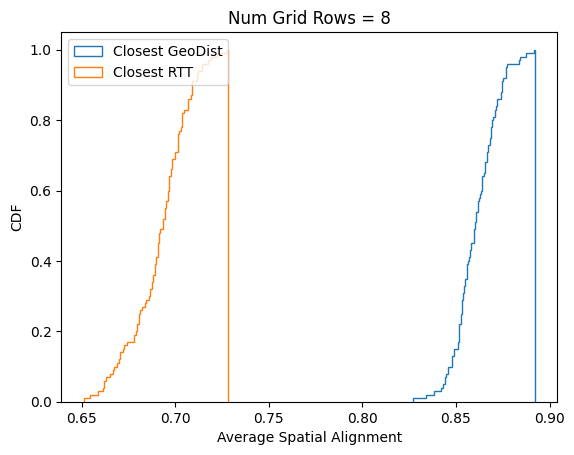
\includegraphics[width=\linewidth]{figures/mechanisms/spatial_ctx_mgmt/spatial_alignment_randomized_8_rows.png}
  \caption{}
\end{subfigure}\par\medskip
\begin{subfigure}{0.45\textwidth}
  \centering
  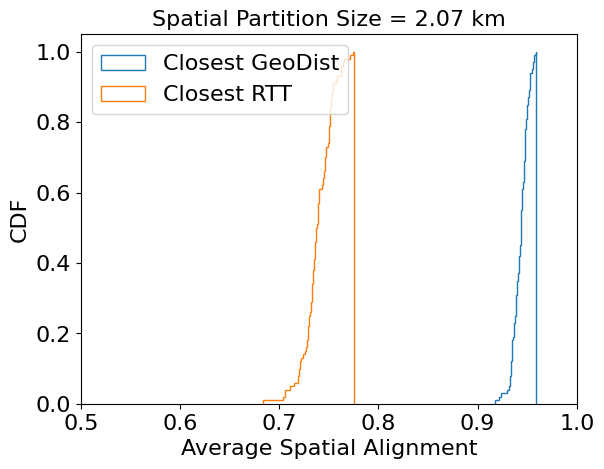
\includegraphics[width=\linewidth]{figures/mechanisms/spatial_ctx_mgmt/spatial_alignment_randomized_16_rows.png}
  \caption{}
\end{subfigure}%
\begin{subfigure}{0.45\textwidth}
  \centering
  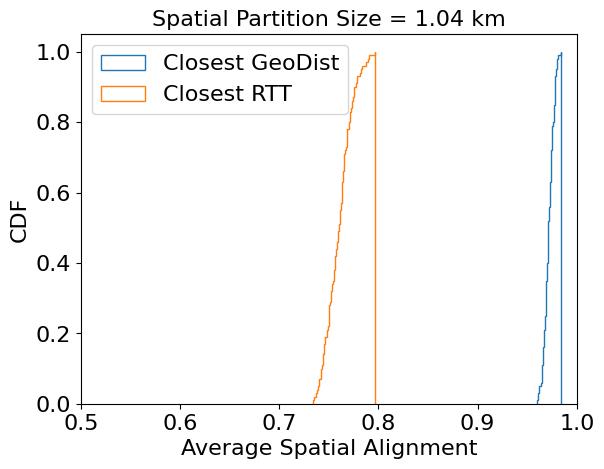
\includegraphics[width=\linewidth]{figures/mechanisms/spatial_ctx_mgmt/spatial_alignment_randomized_32_rows.png}
  \caption{}
\end{subfigure}
\caption{Distribution of Average Spatial Alignment observed for different sizes of each spatial partition. Closest \gls{rtt} based mapping of clients to Edge sites results in worse spatial alignment compared to Closest Geo Distance based mapping. }
\label{fig:spatial_alignment_eval}
\end{figure}

\par \noindent \textbf{Spatial Alignment Evaluation. }To evaluate the above client-to-application mapping baseline heuristics in terms of spatial alignment, we first consider the area of the city under evaluation and divide it into a number of spatial partitions, within which we ideally expect clients to be mapped to the same application instance (thereby creating a perfect spatial alignment). The size of spatial partitions is varied in the experiment to represent a diverse set of applications. We create 1000 clients (with equal number of clients connected to each network provider) and place each one of them at a cell tower location. The placement of clients at cell tower locations is justified by the fact that the spatial distribution of cell towers follows that of client activity. This client placement is randomized and the experiment is repeated 100 times. For each experiment run, we compute the average spatial alignment over all spatial partitions in the scenario. \cref{fig:spatial_alignment_eval} shows the distribution of the average spatial alignment that results from mapping clients to application instances using greedy heuristics that aim at minimizing geographical distance and network \gls{rtt} between the client and Edge site. The metric shown is average spatial alignment, that is the average of the spatial alignment of all the spatial partitions in that experiment run. Although the baseline policy GeoDist, that selects the geographically closest Edge site, is able to attain a high enough average spatial alignment, it does not attain the perfect 1.0 value because not all clients in a given spatial partition always have the same Edge site as the closest. Furthermore, the Closest RTT approach offers even worse spatial alignment because often within a given spatial partition, clients that belong to two different network providers may be bound to different Edge sites. 

\begin{figure}
\centering
\begin{subfigure}{0.3\textwidth}
  \centering
  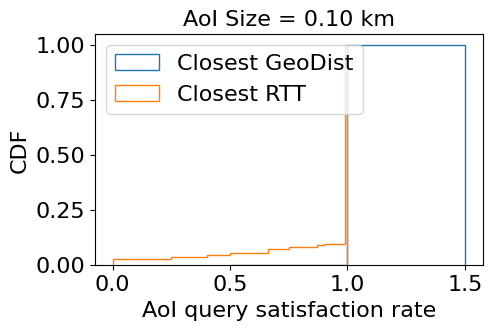
\includegraphics[width=\linewidth]{figures/mechanisms/spatial_ctx_mgmt/aoi_satisfaction_rate_cdf_AOI_0_100_km.png}
  \caption{}
\end{subfigure}%
\begin{subfigure}{0.3\textwidth}
  \centering
  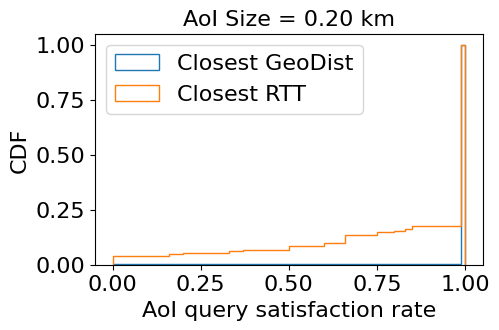
\includegraphics[width=\linewidth]{figures/mechanisms/spatial_ctx_mgmt/aoi_satisfaction_rate_cdf_AOI_0_200_km.png}
  \caption{}
\end{subfigure}
\begin{subfigure}{0.3\textwidth}
  \centering
  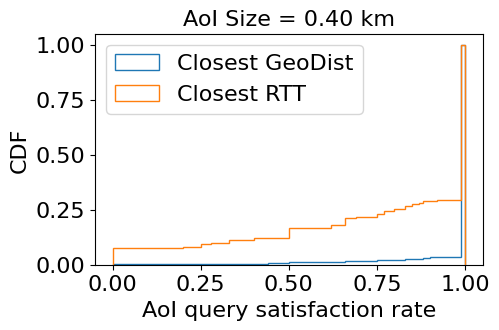
\includegraphics[width=\linewidth]{figures/mechanisms/spatial_ctx_mgmt/aoi_satisfaction_rate_cdf_AOI_0_400_km.png}
  \caption{}
\end{subfigure}
%\par\medskip
\begin{subfigure}{0.333\textwidth}
  \centering
  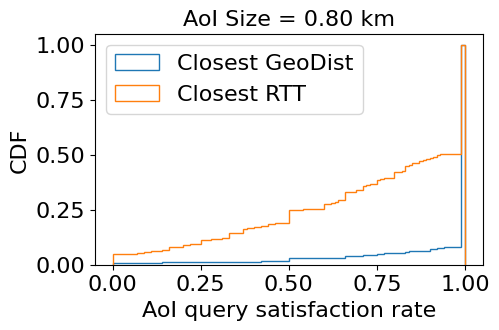
\includegraphics[width=\linewidth]{figures/mechanisms/spatial_ctx_mgmt/aoi_satisfaction_rate_cdf_AOI_0_800_km.png}
  \caption{}
\end{subfigure}%
\begin{subfigure}{0.333\textwidth}
  \centering
  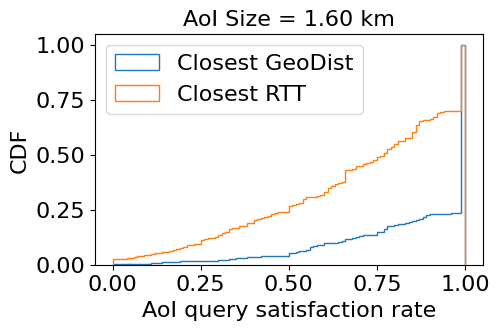
\includegraphics[width=\linewidth]{figures/mechanisms/spatial_ctx_mgmt/aoi_satisfaction_rate_cdf_AOI_1_600_km.png}
  \caption{}
\end{subfigure}%
\begin{subfigure}{0.333\textwidth}
  \centering
  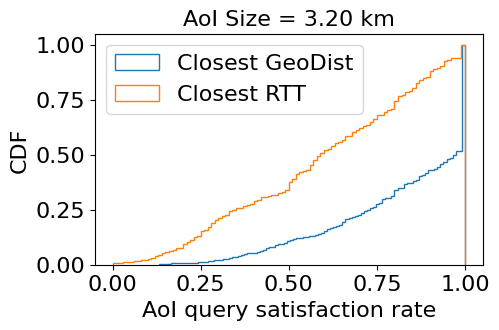
\includegraphics[width=\linewidth]{figures/mechanisms/spatial_ctx_mgmt/aoi_satisfaction_rate_cdf_AOI_3_200_km.png}
  \caption{}
\end{subfigure}
\caption{Distribution of the \gls{aoi} Satisfaction Rate achieved when using two baseline client-to-site mapping approaches - Closest GeoDist and Closest RTT. Both approaches fail to achieve perfect \gls{aoi} Satisfaction Rate especially at higher \gls{aoi} Sizes.}
\label{fig:aoi_satisfaction_rate_eval}
\end{figure}

\par \noindent \textbf{AoI Satisfaction Evaluation.} Next, \cref{fig:aoi_satisfaction_rate_eval} shows the distribution of \gls{aoi} query satisfaction rates offered by the Closest GeoDist and Closest RTT baseline policies for retrieving the data-items with spatial context overlapping with the \gls{aoi} of the querying client. For this evaluation, we consider the scenario wherein each client is associated with one data stream, that contains the sensor data collected by the client. Each client has a dedicated application instance that processes its sensor data, while also consuming the data stream of other clients in its \gls{aoi}. We create one client at every cell tower location, and each client's application instance submits an \gls{aoi} query to find which other clients are in its \gls{aoi}. Depending on the client-to-site mapping, a variable number of \gls{aoi} members are returned, that is compared with the ground-truth set of clients within the \gls{aoi} to compute the query satisfaction rate. The size of \gls{aoi} query is varied to represent a diverse set of applications and their satisfaction rate distributions are shown. Both client-to-site mapping approaches perform poorly and fall significantly short of the expected \gls{aoi} Query Satisfaction Rate of 1.

\par Both of the above approaches fall short in terms of providing high Spatial Alignment for client-to-application mapping and \gls{aoi} Query Satisfaction Rate for serving \gls{aoi}-based queries. The evaluated approaches fall short because they do not incorporate the spatial context of application instance and data-items nor the \gls{aoi} of clients. Instead they rely solely on the client-to-Edge-site mapping, wherein the Closest GeoDist approach is based on the locations of clients and Edge sites, while the Closest RTT approach is based on the network infrastructure topology serving clients and Edge sites. Therefore, we need a new mechanism that takes into account the spatial context and \gls{aoi} specified by the application to perform client-to-application mapping and serving range queries. The mechanism should be able to associate unique spatial contexts to application instances and map clients to these instances based on client location. It should also maintain a spatial index of data-items and filter out the result of an \gls{aoi}-based query by determining which data-items fall within the \gls{aoi}.

\subsection{A New Mechanism for Spatial Context Management}
The Dynamic Spatial Context Management mechanism is utilized by both the control plane's compute and data placement policy of platform services as well as the client library of the platform service running on the client application. The control policy interacts with this mechanism to maintain the spatial context of the system entities (data and compute) while the client library uses this mechanism to keep track of the spatial context of clients. Both these types of spatial contexts are useful in determining which compute/data entities a given client should access. 
\subsubsection{Interface exposed to the control plane}
\par The mechanism divides the geographical space into rectangular regions called \textit{Tiles}, that are of arbitrary size. We choose rectangular tiles so that they can best approximate the spatial partitions expected by collaborative situation-awareness applications. An example partitioning is shown in \cref{fig:aoi_range_partition}. Each Tile has a unique Tile ID, that can be used to directly reference the Tile. Each tile contains a number of entities, such as clients or data-items within it. In the following list, we enumerate the various functions that the mechanism exposes to the control plane for accessing and updating the spatial partitioning.
\begin{itemize}
\item \textbf{GetTileID}. This function is used to convert a location to the ID of the tile that it belongs to. The function is used by the control plane policy to perform client-to-application mapping.
\par \noindent \textbf{Input:} Location of the client
\par \noindent \textbf{Returns: }ID of the tile within which the client location exists.
\item \textbf{GetTileCoverage}. This function determines the bounding box of the spatial area covered by a given tile. This function is used by the control plane policy to perform client-to-application mapping as well as by the libraries on the client and application components to detect if a change of mapping is needed in the event of significant client mobility. 
\par \noindent \textbf{Input: }ID of the tile.
\par \noindent \textbf{Returns: }Bounding box that represents the spatial area covered by the tile.
\item \textbf{UpdateEntityLocation}. This function is used to update the location of an entity, that could be a client or a data-item. In addition, if the new location of the entity is in a different tile than its previous location, this function would move the entity from previous tile to the new tile. 
\par \noindent \textbf{Input: }ID of the entity and its current location.
\item \textbf{GetIntersectingTiles}. This function is used by the client and application component library to perform range queries to find out which entities are within a given geographical  range. 
\par \noindent \textbf{Input: } Bounding box of the area within which to query for intersecting tiles.
\par \noindent \textbf{Returns: } A set of tiles that intersect with the provided bounding box.
\item \textbf{SplitTile}. This function call is used by the control plane to split a tile into two. The split is carried out in a way to ensure that the number of entities in the two resultant tiles is (almost) equal. This function is used to alleviate load on a tile that is going through a workload surge.
\par \noindent \textbf{Input: } ID of the tile to be split.
\par \noindent \textbf{Returns: } IDs of the children tiles created by splitting input tile.
\item \textbf{MergeTiles}. This function allows the control plane to trigger a merging of two adjacent tiles. This function is called when the tiles being merged are experiencing workload under-utilization, and their total workload can be handled by one tile along.
\par \noindent \textbf{Input: } IDs of the tiles to merge.
\par \noindent \textbf{Returns: } ID of the tile created as a result of merging input tiles.
\end{itemize}

\subsubsection{Demonstration of using the mechanism for implementing a control plane policy}
We now demonstrate how the proposed mechanism and the associated API are useful in implementing control plane policies for platform services. For this mechanism, we use an application orchestrator as the driving example. \cref{algo:deploy_req} shows the pseudocode of the control plane policy for finding a suitable application instance for mapping a client based on its geographical location and the spatial contexts of various region-level application instances. The control plane maintains a mapping $APPS$ between an application instance and the Tile that represents the geographical area served by the application instance. The policy first determines the Tile in which the client is currently located. If the client's tile already has an application instance associated with it, the policy returns connection information about that instance. Otherwise the policy deploys a new application instance for the client's tile, maps the application instance to the tile and returns its information to the client. The policy also adds the client to the tile to update the occupancy information, that can be used to detect overload and trigger re-partitioning.
\begin{algorithm}
\caption{Handling Deploy Request from Client}
\begin{algorithmic}
\Require client $c$
\Require client's location $loc$
\State $t \gets GetTileID \left( loc \right)$
\If{$APPS \left[ t \right] exists$}
    \State $A \gets APPS \left[ t \right]$
\Else
    \State Deploy app component $A$ for tile $t$
    \State $APPS  \left[ t \right] \gets A$
\EndIf
\State $UpdateEntityLocation \left(t, c \right)$
\State $SendConnectionInfo \left(c, A \right)$ \Comment{Send info to client for connecting to app component}
\end{algorithmic}
\label{algo:deploy_req}
\end{algorithm}

\cref{algo:handle_overloaded} describes the control plane policy for handling an overloaded region-level component due to workload skew. This policy is triggered by the control plane when it identifies that a given application instance is overloaded by the compute requirement of serving all the clients that are currently present in the tile its is mapped to. Hence, the tile needs to be split and workload divided among two application instances. The policy takes as input the tile associated with the overloaded application instance. The policy uses the \textit{SplitTile} function to create two new tiles. It reuses the application instance for the old tile for one of the new ones, and deploys another instance for the second new tile. Each client that belonged to the old tile is now a part of one of the two new tiles. The policy sends the connectivity information of the new application instances to the respective clients. Although not shown, the \textit{MergeTiles} functionality provided by the mechanism can be similarly used to merge two tiles together if the two application instances serving these two tiles are sufficiently underutilized.
\begin{algorithm}
\caption{Handling an Overloaded Tile}
\begin{algorithmic}
\Require overloaded tile $t$
\State $t1, t2 \gets SplitTile \left( t \right)$
\State $APPS \left[ t1 \right] \gets APPS \left[ t \right]$
\State Deploy app component $A$ for tile $t$
\State $APPS  \left[ t2 \right] \gets A$
\For{client $c \in GetEntities \left( t1 \right)$}
    \State $SendConnectionInfo \left(c, APPS \left[ t1 \right] \right)$
\EndFor
\For{client $c \in GetEntities \left( t2 \right)$}
    \State $SendConnectionInfo \left(c, APPS \left[ t2 \right] \right)$
\EndFor
\end{algorithmic}
\label{algo:handle_overloaded}
\end{algorithm}

\subsubsection{Improvement over Previous Approaches}
In \cref{sec:spatial_ctx_prev_work}, we have shown how the previous work in mapping clients to application instances and serving Area-of-Interest-based queries fall short in terms of meeting the spatial affinity requirements of situation-awareness applications. Here we briefly show the benefit of using a mechanism for maintaining client-to-application mapping based on the spatial context of application instances and location of clients. The details of the mechanism are presented in \cref{sec:spatial_ctx_dse}. We simulate the mobility of 200 clients and use the spatial context management mechanism to map clients to application instances. We measure the spatial alignment over time and plot it in \cref{fig:spatial_alignment_summary}.
\begin{figure}
\centering
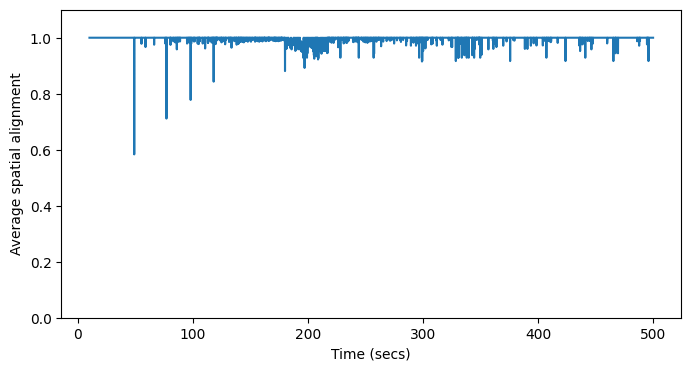
\includegraphics[width=0.75\linewidth]{figures/mechanisms/spatial_ctx_mgmt/spatial_alignment_vs_time.png}
\caption{Spatial Alignment over time. The dips in spatial alignment are due to updates to the spatial partitioning as well as clients moving from one spatial partition to the other and the control plane taking some time to update the client-to-application mapping.}
\label{fig:spatial_alignment_summary}
\end{figure}
The spatial alignment offered by the proposed mechanism remains close to 1.0 for most of the time, with the exception of some dips which are caused either due to dynamic updates to the spatial partitioning by the mechanism or due to the control plane taking some time to update the client-to-application mapping when clients move to different spatial partitions. \cref{fig:spatial_alignment_cdf} shows the behavior of spatial alignment metric more clearly, wherein we can see that for the vast majority of time instants the spatial alignment value is a perfect 1.0. Therefore, the use of a mechanism that explicitly maintains the spatial context of application instances and uses the geographical location of clients to map them to application instances can satisfy the spatial affinity requirements of applications.
\begin{figure}
\centering
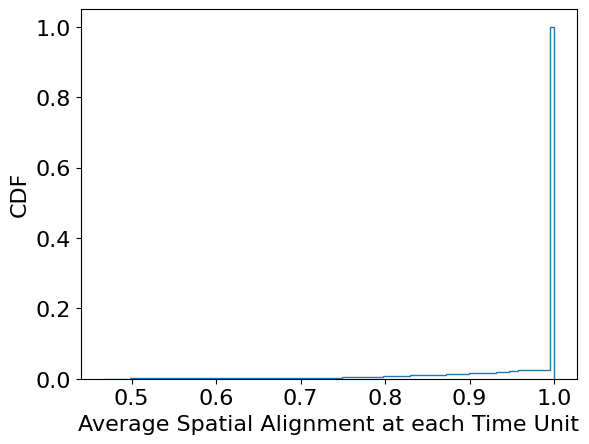
\includegraphics[width=0.5\linewidth]{figures/mechanisms/spatial_ctx_mgmt/spatial_alignment_cdf.png}
\caption{\gls{cdf} of Spatial Alignment values over all time instants. Each data point in the \gls{cdf} corresponds to a point in \cref{fig:spatial_alignment_summary}.}
\label{fig:spatial_alignment_cdf}
\end{figure}
\section{Network Proximity Estimation}
The critical path of applications' control-loop contains system entities (e.g., clients and application components) communicating with one another and accessing data-items. In a densely geo-distributed and heterogeneous infrastructure such as the Edge, the network latency between a client and an Edge site varies significantly depending on which site the client is communicating with. Similarly, the network latency between different Edge sites is also heterogeneous (as discussed in \cref{sec:nw_prox_prev_work}). Hence the choice of Edge site for hosting compute or data components of an application instance has a significant effect on the perceived end-to-end latency of the application, be it the sense-process-actuate control-loop's latency or the latency of accessing data from other clients for inter-client coordination \cite{sarkar2016theoretical,amarasinghe2018data,naas2017ifogstor,liu2019mobility}. Therefore, placement policies in the control plane of platform services need to be aware of the topology of the underlying infrastructure to make decisions. For instance, in the case of the collaborative perception application, the placement of application components should be such that the end-to-end processing latency is bounded under the application's  threshold. Similarly, in the case of the drone swarm coordination application, the publish-subscribe topic should be placed on a suitable broker node to ensure that the end-to-end message delivery latency is bounded under the application's threshold.  
\par Therefore, the platform services require a mechanism that enables their control plane to estimate the network latency between the end-clients and Edge sites as well as across Edge sites. Such a mechanism would be able to estimate the network latency between a pair of entities quickly and with low overhead, making it suitable to be used as a part of the placement policies of these platforms that evaluate a number of Edge sites as candidates for compute or data placement. Given the dynamic nature of the Edge infrastructure and client mobility, the network proximity estimation should also be able to adapt to dynamic changes in network latency between system entities.

\subsection{Control plane policies that need this mechanism}
Network proximity estimation is useful for control plane policies that map logical system entities, such as application instances or publish-subscribe topics, to physical nodes in a way that the end-to-end latency requirements of applications are met. Previous works in this space \cite{amarasinghe2018data,naas2017ifogstor,liu2019mobility} rely on inter-node communication latency estimates for making these decisions. However they do not go into detail about how these estimates are obtained, assuming instead that they are readily available for use by the policy. In the case of the application orchestrator platform service, that manages situation-awareness applications that consist of a pipeline of multiple components \cite{ananthanarayanan2017real,das2018edgebench}, the end-to-end latency is the sum of the processing latency at each application component and the communication latency between each upstream-downstream pair of components. Similarly, in the case of a publish-subscribe system, the end-to-end messaging latency for a given topic is the sum of the communication latency from the publisher clients to the broker, the processing latency on the broker and the communication latency from the broker to the subscriber clients. In the above two systems, estimating the processing latency of application components and publish-subscribe broker can be done using previous works in the cloud computing realm as well \cite{khare2018scalable}. However, estimating the communication latency between a pair of nodes requires rethinking and potentially coming up with a new mechanism. Both the resource allocation policy for the application orchestrator and topic placement policy for publish-subscribe system would benefit from such a new mechanism.

\subsection{Limitations of previous work in proximity-aware compute/data placement}
\label{sec:nw_prox_prev_work}
Control plane policies for ensuring that compute and data entities accessed by a given set of clients is placed in their proximity have been one of the main directions of previous research in Edge computing. The use of geographical distance as a proxy for network latency has been commonly used, given the simplicity of the scheduling logic once the geo-locations of system entities (e.g., clients and edge sites) are known. Sarkar and Misra \cite{sarkar2016theoretical} propose the transformation of geographical distance between a client and candidate Edge site into the network latency between them using a linear transformation $rtt\left(ms\right) = dist \left(km\right) * 0.02 + 5$ \cite{qureshi2010power}. Other works do not rely on the use of such a transformation, but rather perform greedy placement on the geographically closest site to ensure low-latency access to the data or compute entity \cite{lahderanta2021edge}. Geographical location has also been used in a more coarse-grained manner, in that the placement of compute/data entities is specified to be within a large location, e.g., within a city \cite{vilaccageolocate}. The selection of the specific Edge site is done on the basis of a second order policy logic that aims to ensure even load distribution among the various Edge sites in that particular coarse-grained geographical area. 
\par The above approaches fail to work in realistic edge settings because they assume that geographical proximity is correlated with network proximity, which is not true because of lack of uniformity in the way in which different network providers are peered with each other. Two systems entities (a client and an Edge site, or two Edge sites) in close physical proximity might have to communicate through extended routing paths because of the peering between the network providers serving the two entities. In \cref{fig:geodist_vs_rtt}, we present the variation of network round-trip times between an Edge site located in Shanghai to other Edge sites throughout China. It shows that although network latencies are loosely correlated with geographical distance, there is a significant amount of variance, that will result in placement policies choosing an incorrect Edge site for hosting a compute or data entity. In \cref{fig:same_city_diff_prov}, we specifically measure the network round-trip times between sites that are located in the same city, but are served by different network providers. The high round-trip times implies that the high variation in \cref{fig:geodist_vs_rtt} is due to the expensive peering between different network providers hosting Edge sites. 
\begin{figure*}[t!]
    \centering
    \begin{subfigure}[t]{0.45\textwidth}
        \centering
        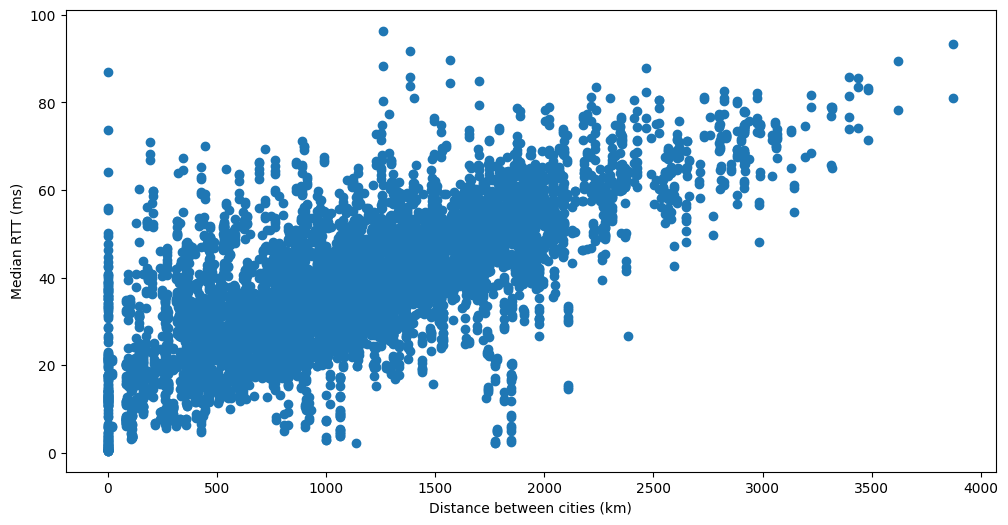
\includegraphics[width=\textwidth]{figures/mechanisms/nw_proximity/shortest-rtt-vs-dist.png}
        \caption{Variation of network \gls{rtt} with geographical distance between Edge Sites.}
        \label{fig:geodist_vs_rtt}
    \end{subfigure}%
    ~ 
    \begin{subfigure}[t]{0.45\textwidth}
        \centering
        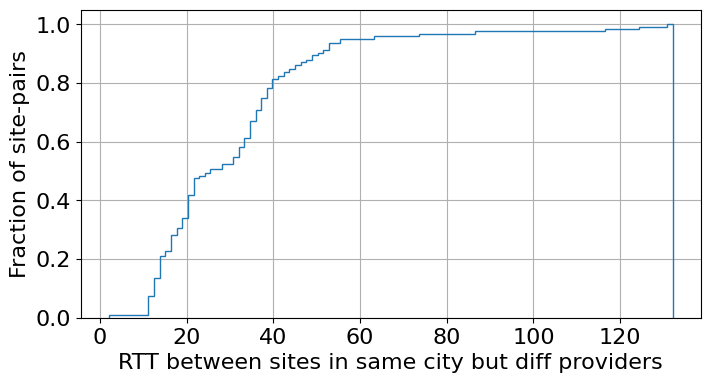
\includegraphics[width=\textwidth]{figures/mechanisms/nw_proximity/same_city_diff_provider_rtts.png}
        \caption{Client-Site \gls{rtt} for sites selected by transforming the geographical distance into network \gls{rtt} and uniformly choosing one among the set of sites satisfying the latency constraint.}
        \label{fig:same_city_diff_prov}
    \end{subfigure}
    \caption{Variation of network \gls{rtt} between edge sites with respect to geographical distance.}
\end{figure*}

\begin{figure*}[t!]
    \centering
    \begin{subfigure}[t]{0.45\textwidth}
        \centering
        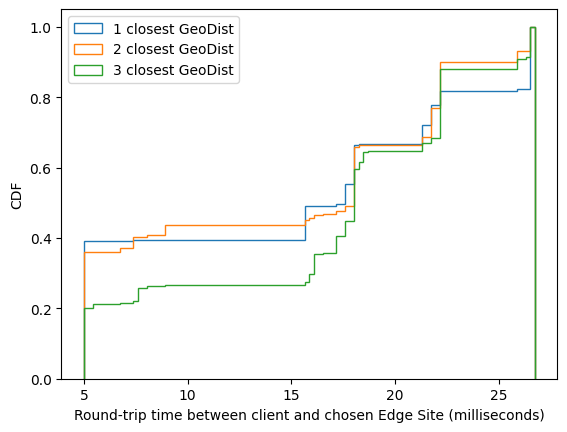
\includegraphics[width=\textwidth]{figures/mechanisms/nw_proximity/geodist_greedy.png}
        \caption{Client-Site \gls{rtt} for sites selected by Greedy approaches. In the case that the closest site is overloaded, the next closest site is considered and so on.}
        \label{fig:geodist_greedy}
    \end{subfigure}%
    ~ 
    \begin{subfigure}[t]{0.45\textwidth}
        \centering
        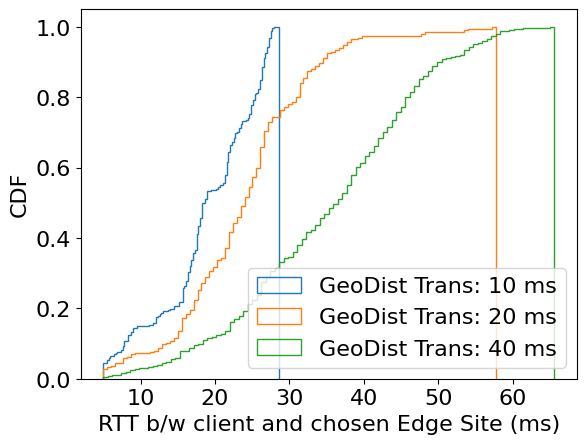
\includegraphics[width=\textwidth]{figures/mechanisms/nw_proximity/geodist_trans_rtt.png}
        \caption{Client-Site \gls{rtt} for sites selected by transforming the geographical distance into network \gls{rtt} and uniformly choosing one among the set of sites satisfying the latency constraint.}
        \label{fig:geodist_trans}
    \end{subfigure}
    \label{fig:baseline_proximity_policies}
    \caption{Performance of Edge Site selection approaches that rely on geographical distance as a proxy for network proximity.}
\end{figure*}

\par We evaluate the efficacy of the aforementioned baseline proximity estimation techniques - the greedy distance-minimization approach and the one that transforms geographical distance to network \gls{rtt}. For this experiment, we consider the infrastructure topology of the city of Shanghai as described in \cref{sec:nep_infra_topology}. We simulate clients at randomly (uniformly) chosen cell tower locations and aim to find an Edge site to host its application instance using one of the above two policies. The goodness of an Edge site selection is quantified by the observed \gls{rtt} between the client and chosen Edge site. 
\par The Greedy policy always selects the closest Edge site in terms of geographical distance between the client and the site. In case the chosen Edge site is undergoing compute overload, the policy selects the next closest site, and so on. The other site selection policy that we evaluate is one that transforms the geographical distance between client and Edge site to network round-trip time and uses this estimate to filter out those sites that can meet the latency bound imposed by the application. Among the filtered sites, the policy uniformly selects one so as to minimize workload skews.
\par \cref{fig:geodist_greedy} shows the observed \gls{rtt} when selecting a site using the greedy approach. For more than 50 percent of the clients, the geographically closest site is not the one that it is directly connected to over the network, and hence, traffic needs to go through the network provider's core, or through the Internet to get to it. Since there is no strict correlation between geographical distance and network \gls{rtt}, this behavior is similar for second and third closest sites as well. For the distance-\gls{rtt} transformation based approach, we compare the site selection with an application-imposed \gls{rtt} bound of 10, 20 and 40 milliseconds. We see however, that the transformation does not sufficiently filter out infeasible sites and a large majority of clients have the latency bound violated.
\par The key takeaway from the above experiments is that both the above approaches that use geographical distance between system components to estimate network proximity fail to fulfill their objective of selecting an Edge site that has low communication latency from the client. The fundamental flaw with them is that they overlooks a key property of real-world network topologies, in that the network route taken by packets seldom aligns with the geographically shortest path between the source and destination entities. Furthermore, there are additional delays caused at the various intermediate hops. Hence, we need a new mechanism for network proximity estimation that derives the proximity information from actual measurement of the network latency between system entities.

\subsection{A New Mechanism for Network Proximity Estimation}
We propose a new mechanism for network proximity estimation that computes the proximity estimation based on actual network round-trip time measurements between system entities.
\subsubsection{Interface exposed to the control plane}
All system components of the platform service (clients, worker nodes, data nodes, etc.) are assigned a unique network proximity identifier. The network proximity mechanism then provides the platform service a function \textbf{NetworkRTT} that takes as input the IDs of two system components and returns the estimated network round-trip time between the two components. 

\subsubsection{Using network proximity mechanism for compute/data placement}
\label{sec:policy_using_nw_prox}

We now demonstrate the use of the proposed Network Proximity Estimation mechanism for implementing a control plane policy, specifically the broker selection policy for a publish-subscribe system (\cref{fig:nw_proximity_pubsub_e2e_latency}). This control plane policy selects the broker to host a given topic such that the end-to-end message delivery latency for all publisher-subscriber pairs is under the latency threshold for the topic, as shown in \cref{fig:nw_proximity_pubsub_e2e_latency}. As described in \cref{algo:pubsub_nw_prox_example}, it iterates over all the potential candidate brokers and computes the worst-case communication latency if the topic is hosted on each of those brokers. The worst-case communication latency is the sum of the maximum publisher-broker network latency and the maximum broker-subscriber network latency. The sum of worst-case communication latency and processing latency on the broker gives the worst-case end-to-end latency for that topic. All the brokers that have the worst-case end-to-end latency under the topic-specific threshold are selected as candidates. The policy finally selects the candidate broker currently serving the lowest message rate among all candidates to ensure load balancing among brokers.

\begin{figure}
\centering
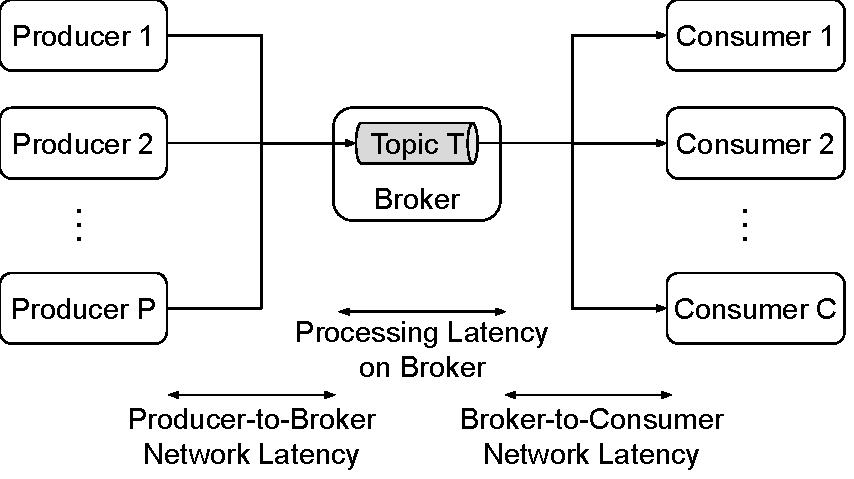
\includegraphics[width=0.6\linewidth]{figures/mechanisms/nw_proximity/pubsub_e2e_latency.pdf}
\label{fig:nw_proximity_pubsub_e2e_latency}
\caption{An instance of publish-subscribe service as an exemplary platform-service that requires information about network communication latency to compute the end-to-end latency experienced by the application. In this example, the end-to-end latency is the message delivery latency from any producer to all consumers for a given topic. The end-to-end latency is given by the sum of the maximum network latency from any producer to the broker, the processing latency on the broker, and the maximum network latency from the broker to any consumer.}
\end{figure}

\begin{algorithm}
\caption{Broker selection policy for topic $T$ with end-to-end message delivery latency threshold $L_{th}$}
\label{algo:pubsub_nw_prox_example}
\begin{algorithmic}
\Require topic $T$
\Require latency threshold $L_{th}$
\State $prod \gets \text{ set of producers for }T$
\State $cons \gets \text{ set of consumers for }T$
\State $candidates \gets \{\}$
\For{$\text{each broker } b$} 
    \State $nw\_lat \gets max_{p \in prod} \dfrac{1}{2} \cdot NetworkRTT \left( p, b \right) + max_{c \in cons} \dfrac{1}{2} \cdot NetworkRTT \left( c, b \right)$
    \State $e2e \gets nw\_lat + proc\_latency \left( b \right)$
    \If{$e2e \leq L_{th}$}
        \State $candidates \gets candidates \cup \{b\}$
    \EndIf
\EndFor
\Return broker in $candidates$ with lowest $msg\_rate$
\end{algorithmic}
\end{algorithm}

\subsubsection{Improvement over Previous Approaches}
We evaluate the performance of the proposed Network Proximity Estimation mechanism by performing an experiment similar to the one described in \cref{sec:nw_prox_prev_work}. We place clients randomly at cell tower locations and aim to find Edge sites within different \gls{rtt} thresholds. In this experiment, the Edge site selection policy utilizes the network proximity between clients and Edge sites to estimate the network \gls{rtt} between them and uses it to filter the suitable sites. \cref{fig:nw_prox_summary_result} shows the distribution of the \glspl{rtt} observed from the Edge site chosen for clients. The Edge site selection policy is able to satisfy all the constraints on \gls{rtt} and outperform the geographical distance based approaches. The design-space exploration of the network proximity estimation mechanism has been discussed in detail in \cref{sec:nw_prox_dse}.
\begin{figure}
\centering
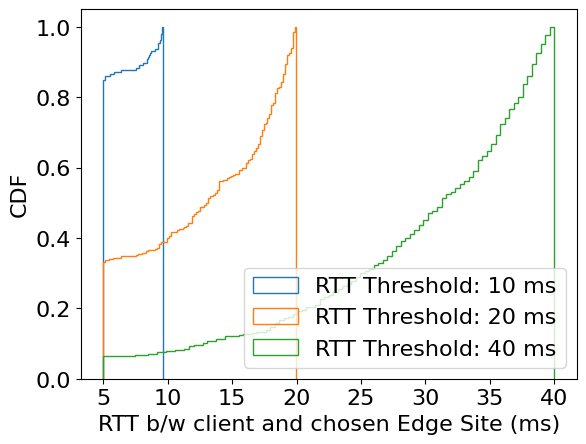
\includegraphics[width=0.5\textwidth]{figures/mechanisms/nw_proximity/nc_rtt_threshold.png}
\caption{Distribution of client-Edge-site \gls{rtt} for different \gls{rtt} constraints when site selection is done by using the Network Proximity Estimation mechanism. The proposed mechanism ensures that the selected Edge sites satisfy the \gls{rtt} constraint.}
\label{fig:nw_prox_summary_result}
\end{figure}

\section{End-to-End Monitoring Mechanism}
\label{sec:monitoring_mechanism}
Thorough monitoring of applications running atop platform services is a non-trivial task because there can be multiple sources of performance violation. For instance, as shown in \cref{fig:pipeline_latencies}, the observed end-to-end latency of the application instance is a sum of the queuing, execution and downstream communication latencies of each operator in the pipeline.  Thus, detecting a violation of the end-to-end latency requirement and identifying the root-cause requires monitoring \new{measurements} of all the component latency metrics as independent \new{streams} \soutnew{timeseries} and their aggregation and analysis. Each platform service has a notion of an \textit{application unit}, that represents an independent set of system entities that do not affect the performance of entities not within the given unit. An example of an application unit is a publish-subscribe topic, that consists of all the producers, consumers and broker hosting that topic. Furthermore, each platform service has its own set of \new{metric streams} \soutnew{metrics} that need to be monitored for each application unit. \new{The measurements from these metric streams}\soutnew{These metrics} then need to be aggregated and analyzed in way that is specific to the platform service for detecting violations. The monitoring mechanism needs to scale with an increasing number of application instances being monitored and impose low overhead on the applications and infrastructure.
\begin{figure}
\centering
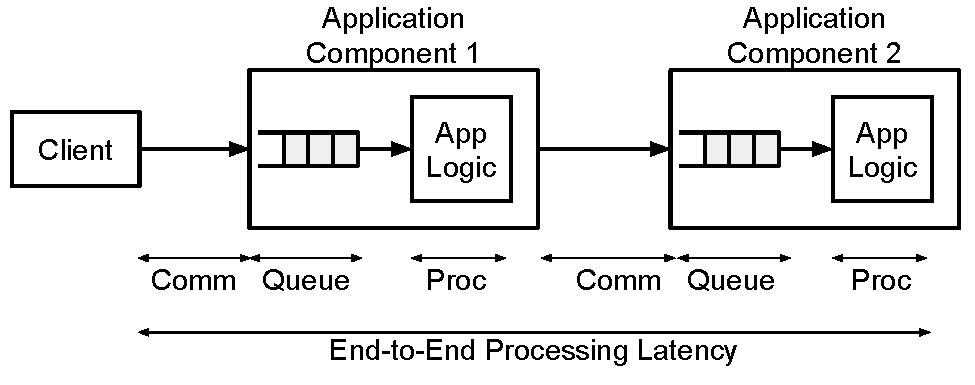
\includegraphics[width=0.75\linewidth]{figures/mechanisms/monitoring/pipeline_latencies}
\caption{A breakdown of the end-to-end processing latency of an application pipeline into its constituent latencies.}
\label{fig:pipeline_latencies}
\end{figure}

\subsection{Control plane policies that need this mechanism}
Situation-awareness applications require that the end-to-end latency requirement is satisfied for the entire lifetime of the application, so that correct functionality can be guaranteed. However, given the constant mobility of end-clients and the stringent latency requirements, their requirements are likely to be violated repeatedly and frequently. For instance, a car moving away for the Edge Site currently serving the vehicle-local processing component would incur higher end-to-end processing latency due to higher communication delays. Hence, the control plane of the platform services are required to constantly monitor the running applications for such violations, perform root-cause analysis for determining the cause of the violation, and take appropriate reconfiguration action(s) to resolve the violation. In the above example, a reconfiguration would involve the migration of the application component to an Edge Site that is closer (in terms of network proximity) to the end-client to ensure end-to-end latency satisfaction.

\subsection{Shortcomings of previous work}
\label{sec:monitor_prev_work}
\par Application monitoring has been an active area of work in the cloud computing space with a number of research projects and commercial offerings available. In the context of cloud computing, applications typically do not possess end-to-end latency requirements and the goal of monitoring is to ensure that the tail latency of a given service (that could consist of multiple application components) does not increase significantly. Prior art such as Prometheus \cite{prometheus} and Monasca \cite{monasca} do not support the aggregation of multiple \soutnew{metrics}\new{metric streams} to study the behavior of end-to-end latency. Furthermore, their architecture is a fully centralized one, resulting in the use of network bandwidth to send the monitoring data to one specific location (e.g., the Cloud).
\par Monitoring systems designed for Edge computing environments also suffer from limitations, wherein they aggregate \new{measurements from metric streams}\soutnew{measured metrics} over geographical regions instead of aggregating multiple \new{metric streams}\soutnew{metrics} pertaining to the same application instance \cite{fmone, gonccalves2021dynamic}. Such systems are not capable of detecting violations of end-to-end latency constraints. Previous contributions to building systems services such as publish-subscribe systems \cite{emma} and distributed application runtimes \cite{foglets} consist of monitoring subsystems that only monitor the the network connectivity between a client and the Edge site that it is connected directly to. Since these solutions do not consider end-to-end latency as the primary metric, they result in triggering more reconfigurations to keep clients connected to the closest Edge site than needed.
\begin{figure}
\centering
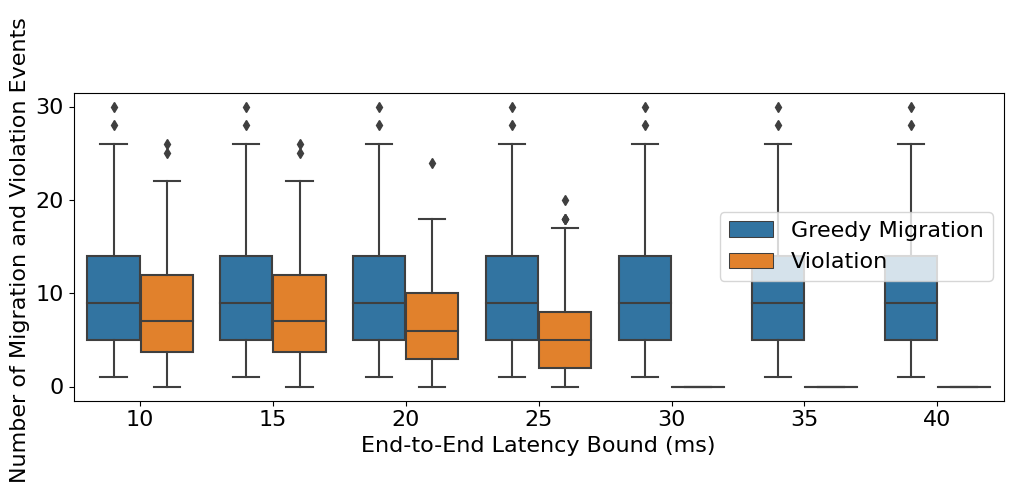
\includegraphics[width=0.75\linewidth]{figures/mechanisms/monitoring/migrations_count_greedy.png}
\caption{Number of migrations triggered by the Greedy monitoring approach along with the actual number violations faced by clients. The end-to-end latency threshold is varied along the x-axis.}
\label{fig:migration_count}
\end{figure}
\par We show an evaluation of a greedy monitoring approach that aims to minimize the last-mile network latency between the client and the Edge site it directly connects to. The metric of interest is the number of migrations triggered by such a policy, which should be compared to the number of times that the application's latency threshold is actually violated - where a migration is indeed necessary. We simulate the mobility of 200 independent clients in the city of Shanghai using the Random Waypoint mobility model and track the number of migrations triggered by the greedy policy. In \cref{fig:migration_count}, we present the migrations triggered by the greedy policy and the number of latency violations for each client with increasing end-to-end latency bound. We see that as the end-to-end latency bound increases, the number of latency violations decreases, but the number of migrations triggered by the greedy policy remains the same. This behavior is explained by the fact that although the greedy policy triggers the same number of migrations as it is independent of the end-to-end latency constraint, the number of latency violations decreases with an increase in the threshold. 
\par The limitations of an approach that considers only a component of the end-to-end latency necessitates that we come up with a mechanism for monitoring the end-to-end latency by analyzing all the component latencies within it. Violation detection needs to be performed for each application-level unit, or application instance, such as a publish-subscribe topic, or one instance of an application pipeline (as shown in \cref{fig:pipeline_latencies}). Hence, \new{measurements from metric streams}\soutnew{metrics} that belong to the same application unit should be aggregated together for violation detection and root-cause analysis to identify the source of the violation.

\subsection{A New Mechanism for End to End Latency Monitoring}
We now present a mechanism for end-to-end latency monitoring that aggregates and analyzes \new{metric streams for multiple components of the end-to-end latency}\soutnew{multiple component latency metrics that make up the end-to-end latency}.
\subsubsection{Interface exposed to the control plane}
The following abstractions are provided to the control plane of a platform service for using the end-to-end monitoring mechanism.
\begin{itemize}
\item \textbf{RegisterAppUnit.} Registration of an Application Unit when it is created. For instance, when a new topic is created in a publish-subscribe system, the topic should be registered as a new Application Unit. The Monitoring mechanism uses the identifier of the application unit to identify the \new{metric streams}\soutnew{metrics} that pertain to it, and perform end-to-end aggregation on them. 
\par \noindent \textbf{Inputs}:
\begin{itemize}
\item AppUnitId: The ID of the application unit being registered.
\end{itemize}

\item \new{\textbf{RegisterMetricStream.}}\soutnew{\textbf{RegisterMetric.}} System components can register custom \new{metric streams}\soutnew{metrics} and publish their measurements. The \new{metric streams}\soutnew{metrics} are annotated with the application unit that they correspond do, as well as custom platform-specific tags. 
\par \noindent \textbf{Inputs}:
\begin{itemize}
\item EntityID: The ID of the entity that this \new{metric stream}\soutnew{metric} pertains to.
\item MetricType: A string value denoting the type of \new{metric stream}\soutnew{metric}, that is used for querying them.
\item AppUnitId: The ID of the application unit that this \new{metric stream}\soutnew{metric} belongs to.
\item Labels: A dictionary containing a set of key-value pairs, each containing a platform-specific information about the \new{metric stream}\soutnew{metric}.
\item ValueSchema: A schema in YAML format that defines the data-structure of measurements for this \new{metric stream}\soutnew{metric}. It is particularly useful for defining complex \new{metric streams}\soutnew{metric}. Primitive datatypes can be represented by a string (e.g., int or str).
\item BucketSize: The size of the bucket for data aggregation.
\item AggregationFunction: The function to use for aggregation. The mechanism should support basic functions such as Mean, Median, Min, Max and percentile values.
\end{itemize}
\par \noindent \textbf{Returns: } A unique identifier for the \new{metric stream}\soutnew{metric}, that can be used to record measurements and query measurements.
\par The following snippet shows an example, that measures the network latency of an instance of the pipeline stage shown in \cref{fig:app_pipeline} to its downstream component. In the given platform service, the application unit that a \new{metric stream}\soutnew{metric} belongs to is the downstream-most application component, or the root component. In this example, the application unit is the application component instance $L_0$. 
\begin{minted}{yaml}
-   entity_id : "L10"
    entity_type: "APP"
    app_unit: "L0"
    metric: "net_latency"
    labels:
        level: 0
    value_schema: float
    bucket_size: 5 secs
    aggr_fn: AVG
\end{minted}
Each metric stream is represented as an ordered sequence of measurements along with their timestamps as shown in \cref{eq:metric_stream}.
\begin{equation}
M = \left[ \cdots , \left( t, v \right) , \cdots \right] \text{ where } 0 < t < \infty
\label{eq:metric_stream}
\end{equation}
The mechanism time-aligns the measurements for a specific \new{metric stream}\soutnew{metric} into well-defined buckets, that is necessary as a pre-processing step before multiple \new{metric streams}\soutnew{metrics} can be aggregated together. Since measurements from different \new{metric streams}\soutnew{metrics} are likely to be recorded at different instants in time, aligning them in time allows measurements from different \new{metric streams}\soutnew{metrics} to be processed together, such that two measurements from different \new{metric streams}\soutnew{metrics} that were collected at roughly the same time can be processed together\footnote{We assume that clock skew between the entities recording measurements is significantly less than the bucket size. This is a reasonable assumption because typical clock skews are not expected to be more than a few 10s of milliseconds}.
\new{This bucket-based time-alignment approach is an approximation of an ideal end-to-end aggregation of component latencies by recording measurements to every data-item generated by the data-plane. Such an ideal approach is infeasible for two reasons: (a) it behooves instrumenting the application components to record latency incurred by data plane actions which is neither desirable nor possible since the application logic is in the purview of the developer; and (b) it will vastly increase the amount of communication incurred by the system for monitoring the end-to-end latency. Therefore, we choose the aforementioned bucket-based approach.}
\cref{fig:time_alignment} illustrates the time alignment of a \new{metric stream}\soutnew{metric} for a fixed size time bucket, and all measurements within a given bucket are aggregated by taking an average over them. The platform service is supposed to provide the bucket size $B$ (in units of time) and the aggregation function $func$ for aggregating a \new{metric stream}\soutnew{metric} $M$. As described in \cref{eq:metric_stream_alignment}, the alignment of a \new{metric stream}\soutnew{metric} involves aggregating all the measurements within a particular bucket interval using the provided aggregation function to form one measurement.
\begin{figure}
\centering
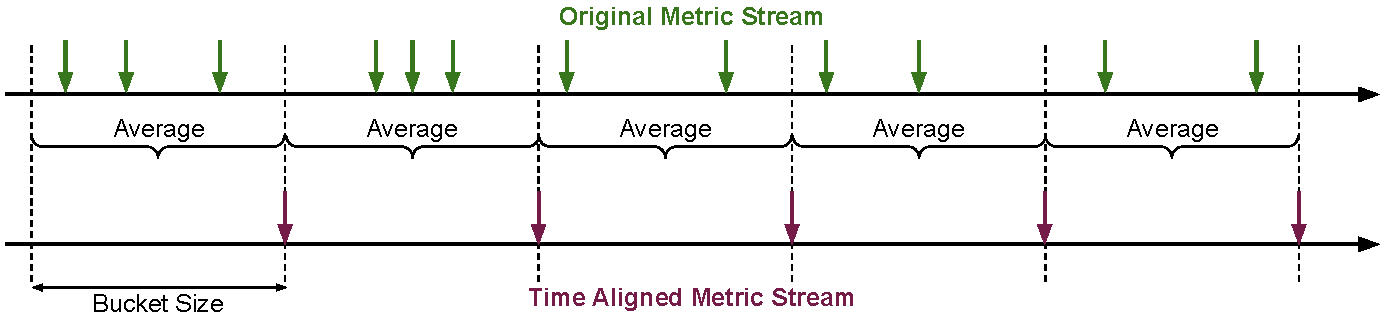
\includegraphics[width=\linewidth]{figures/mechanisms/monitoring/time_alignment}
\caption{Illustration of time alignment of \new{metric streams}\soutnew{metrics}. The individual measurements (denoted by green arrows) within each time bucket are aggregated using the average function to generate the measurement for that bucket (shown by red arrows). The dotted vertical lines indicate the boundaries of buckets. The time alignment function takes as input a metric stream and time bucket size and returns another stream.}
\label{fig:time_alignment}
\end{figure}
\begin{multline}
ALIGN^{func}_{B} \left( M \right) = \left[ \cdots , \left( t, v \right) , \cdots \right] \text{ where } t = n\cdot B \text{ and } 0 < n < \infty \\ \text{ and } v = func \left( \{ v' : \left( t', v'\right) \in M \text{ and } B\cdot \left( n-1\right) < t' \leq n \cdot B \} \right)
\label{eq:metric_stream_alignment}
\end{multline}

\item \textbf{RecordMeasurement.} Platform service components can record measurements for a specific \new{metric stream}\soutnew{metric} using the ID of the entity and the metric \new{stream} type. 
\par \noindent \textbf{Inputs:}
\begin{itemize}
\item MetricID: The ID of the \new{metric stream}\soutnew{metric} that this measurement pertains to.
\item Measurement: A YAML document containing measurement. It can be a nested YAML document in case the metric \new{stream} records complex values.
\end{itemize}
\par The parameters for an example call to the record measurement function are shown below.
\begin{minted}{yaml}
-   metric_id: "net_latency_L0"
    value: 10.0
\end{minted}

%\item Platform-specific definition of the system entity processing all the metrics of a given application unit for performing aggregation and violation detection. For instance, in the case of a publish-subscribe system, all the metrics pertaining to a specific topic can be processed at the broker serving that topic.
\item \textbf{OnNewBucket.} This is a callback function that is called when \new{time-aligned measurements of} all the \new{metric streams}\soutnew{metrics} belonging to a particular application unit are ready for a given bucket. The receiver of this callback is supposed to be an entity in the control plane of the platform service, that receives the end-to-end aggregated view of all the \new{metric streams}\soutnew{metrics} associated with a particular application unit. The control plane entity uses these \new{metric streams}\soutnew{metrics} to make violation detection and reconfiguration decisions.
\par \noindent \textbf{Inputs:}
\begin{itemize}
\item AppUnitID: ID of the application unit that this set of \new{metric streams}\soutnew{metrics} belongs to.
\item Bucket. The timestamp of the bucket that is being reported.
\item Values. A collection of \new{metric streams}\soutnew{metrics} with their metadata and aggregated values for this bucket.
\end{itemize}
\item \textbf{QueryMetrics. }The logic provided to the end-to-end monitoring mechanism via the ProcessMetrics interface should be able to query \new{metric streams}\soutnew{metrics} using their labels. 
\par \noindent \textbf{Inputs:}
\begin{itemize}
\item MetricID: ID of the \new{metric stream}\soutnew{metric} being queried.
\item AppUnitID: ID of the application unit being queried.
\item BucketTimeRange: A range of time within which all buckets for the given \new{metric stream}\soutnew{metric} or application unit need to be returned.
\end{itemize}
\par \noindent \textbf{Returns:} A list of buckets, each containing the timestamp of the respective bucket and a set of values for all the queried \new{metric streams}\soutnew{metrics} for that bucket.

\end{itemize}

\subsubsection{Demonstration of using end-to-end monitoring for control plane policy of a platform service}
In this section, we show how the end-to-end monitoring mechanism will be used for implementing a policy for detecting violations of end-to-end processing latency for application instances running on a geo-distributed Edge infrastructure, as part of the control plane of an application orchestrator. For this example, we restrict the discussion to clients and application instances for a single application unit, but the approach generalizes to multiple application units.
\begin{enumerate}
\item The library of the platform service running alongside each client and backend application instance generates two \new{metric streams}\soutnew{metrics} - namely the processing latency and network latency to the immediately downstream application component instance. For an application component $e$ we denote them as $proc_e$ and $net_e$.\\
\begin{minipage}{0.45\textwidth}
\begin{minted}{yaml}
-   entity_id : "L20"
    entity_type: "CLIENT"
    app_unit: "L0"
    metric: "proc_latency"
    bucket_size: 5 secs
    aggr_fn: AVG
\end{minted}
\end{minipage}%
\hfill
\begin{minipage}{0.45\textwidth}
\begin{tabular}{p{\textwidth}}
\begin{minted}{yaml}
-   entity_id : "L10"
    entity_type: "APP"
    app_unit: "L0"
    metric: "net_latency"
    bucket_size: 5 secs
    aggr_fn: AVG
\end{minted}
\end{tabular}
\end{minipage}

The above listings show definitions of \new{metric streams}\soutnew{metrics} corresponding to the processing and network latency of the application component instance $L_{20}$ and $L_{10}$ respectively in the application instance shown in \cref{fig:app_pipeline}. Both these component latencies pertain to the application unit that is associated with the ``root'' application component instance $L_0$. The platform service requests for time-alignment of all the metric streams using the function $ALIGN^{AVG}_{5secs}$. 
\item The control plane policy for detecting violations of end-to-end processing latency receives the callback \textbf{OnNewBucket} for the application unit $L_0$ as soon as a new bucket for all \new{metric streams}\soutnew{metrics} belonging to it are available. 

\begin{comment}
performs calculations for each of the root application instances, that we denote as $L_0$. It selects the latency metrics corresponding to the clients that are connected to $L_0$ as shown in \cref{fig:app_pipeline}. It uses a query like the following to select the latency metrics for all the clients that are connected to the root application component $L_0$.
\end{comment}

\begin{minted}{sql}
SELECT METRICS WITH
                entity_type="CLIENT" AND app_unit="L0"
\end{minted}

\begin{figure}
\centering
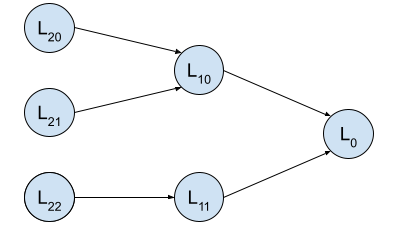
\includegraphics[width=0.5\textwidth]{figures/mechanisms/monitoring/app_pipeline.png}
\caption{Schematic of a typical situation-awareness application. The application model resembles a tree, with the leaf vertices corresponding to clients. Each vertex that is not a leaf is an application instance running on the backend infrastructure (Edge-Cloud continuum). Each vertex processes data generated by the upstream vertices and sends its output data to the downstream vertex (if any).}
\label{fig:app_pipeline}
\end{figure}
\item The above set of \new{metric streams}\soutnew{metrics} are then grouped by the field $entity\_ID$ because they contain measurements for both processing latency and network latency for each client. Grouping them by $entity\_ID$ allows the policy to separate the \new{metric streams}\soutnew{metrics} of a specific entity from other entities.
\item For each client component $c$, the policy computes the set of application components $S_c$ that process data generated by $c$. The following pseudocode illustrates this computation.
\begin{algorithmic}
\State $n \gets c$
\State $S_c \gets \{\}$
\While{$n \neq \phi$} 
    \State $S_c \gets S_c \cup \{ n \}$
    \State $n \gets M \left[ n \right]$
\EndWhile
\end{algorithmic}
We use the notation $M \left[ n \right]$ to denote the downstream application component reading the output of $n$. The downstream application component for the root component $L_0$ is designated to be null ($\phi$). This information is obtained from the application orchestrator platform service's control plane metadata about application mapping.

\item For each client $c$, now it is possible to compute a time-aligned metric stream that records the end-to-end processing latency for $c$.
\begin{equation}
E2E_c^* = \sum_{e \in S_c} proc_e^* + net_e^*
\end{equation}
For those clients whose end-to-end latency estimation exceeds the application's threshold, a reconfiguration action is triggered. The objective of the reconfiguration action is determined by root-cause analysis, that is performed by the platform service's control plane policy itself (described in more detail in \cref{sec:oneedge_root_cause_chapter}). 
\par Briefly, the root-cause analysis analyzes the historical trend of each component latency that makes up the end-to-end latency (i.e., processing and communication latency of each component). It determines the relative contribution of each of the component latencies toward the end-to-end latency violation. In case the violation is most significantly caused by an increase in communication latency between an upstream-downstream application component pair $\left( l1, l2 \right)$ then $l1$ is re-mapped to another downstream component instance that offers  better network latency. Similarly, if the root-cause is an increase in processing latency at a certain component instance $l$, then its resource allocation is increased to bring down the processing latency. If resource allocation cannot be increased due to capacity constraints, a fraction of its immediately upstream component instances are mapped to another instance so as to reduce the workload on $l$. 
\end{enumerate}

\subsubsection{Improvement over Previous Approaches}
We evaluate the improvements brought about by incorporating the end-to-end latency monitoring mechanism into the monitoring policy. We perform the same experiment as in \cref{sec:monitor_prev_work}, with the difference being that the monitoring policy now uses the end-to-end latency estimate from the monitoring mechanism to detect violations. \cref{fig:migration_count_e2e} shows the variation of number of migrations and number of violations experienced by each client during the experiment. Both these metrics are identical because the end-to-end monitoring mechanism triggers a migration only when the end-to-end latency constraint is violated. Therefore no unnecessary migrations are triggered by the monitoring policy. A detailed design space exploration of the end-to-end monitoring mechanism will be discussed in \cref{sec:e2e_mon_dse}.
\begin{figure}
\centering
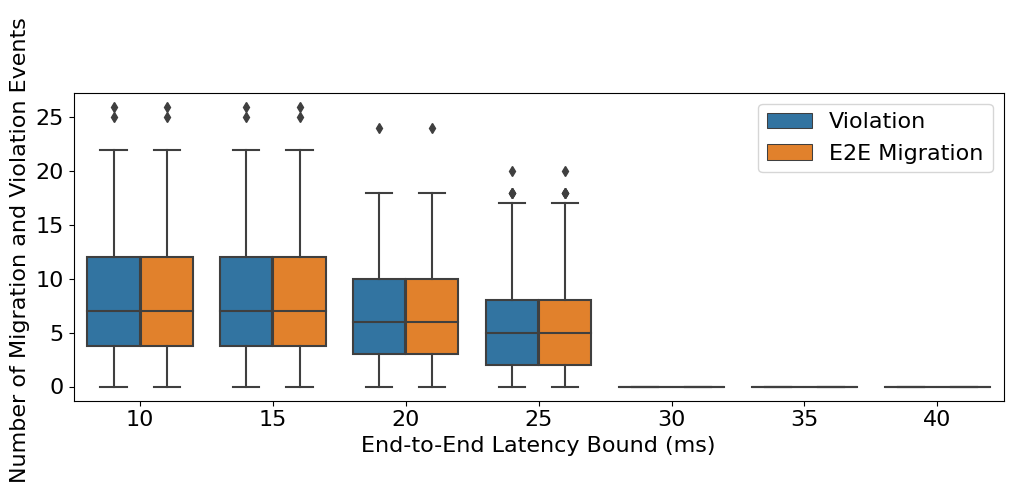
\includegraphics[width=0.75\linewidth]{figures/mechanisms/monitoring/migrations_count_e2e.png}
\caption{Number of migrations triggered by a monitoring approach that utilizes the end-to-end monitoring mechanism for detecting violations. Also shown are the actual number violations faced by clients. The end-to-end latency threshold is varied along the x-axis.}
\label{fig:migration_count_e2e}
\end{figure}

\par \noindent \textbf{Summary.} This chapter presented three mechanisms that are needed by the control plane of platform services to efficiently operate on the Edge. The previous approaches of providing the functionality of these mechanisms are deficient, because of which we propose to design new mechanisms for the same. We propose the following new mechanism: (1) a dynamic spatial context management mechanism; (2) a network proximity estimation mechanism; and (3) an end-to-end latency monitoring mechanism. This chapter introduces the mechanisms, the interface they offer to the control plane policies and a summary of the improvements they can have on the functionality of control plane policies. We will discuss detailed design-space exploration for all three mechanisms in the next chapter.